This section reports the end-to-end results from the updated early-window pipeline using (i) residualized structural shape descriptors, (ii) Hawkes-style dynamic parameters, and (iii) structure--tempo interaction terms. The main analysis is conducted on FibVID in size-based windows ($k \in \{10,20,30,45,60,90,120,180\}$), which hold early volume fixed by design. Twitter15/16 are then used as a comparative benchmark, and time-window results are reported as robustness checks.

\subsection{FibVID Main Results in Size-Based Windows}
Figure~\ref{fig:k_veracity_main} and Figure~\ref{fig:k_reach_main} show the full trajectory across $k$ for FibVID veracity (AUC) and reach ($R^2$). Here, \emph{structure-only} denotes residualized structural shape features only (no tempo, dynamics, or interaction terms): this ablation isolates structural incremental signal and helps avoid treating volume effects as structure effects. At each fixed window, the gaps baseline$\rightarrow$structure-only and structure-only$\rightarrow$full/interaction-full are interpreted as incremental value from structure, then from added dynamics/interactions. The horizontal axis is window size $k$ and the vertical axis is performance (AUC or $R^2$, higher is better); colored lines are feature bundles and error bars are 95\% CIs from SE over fixed CV folds.

\begin{figure}[htbp]
  \centering
  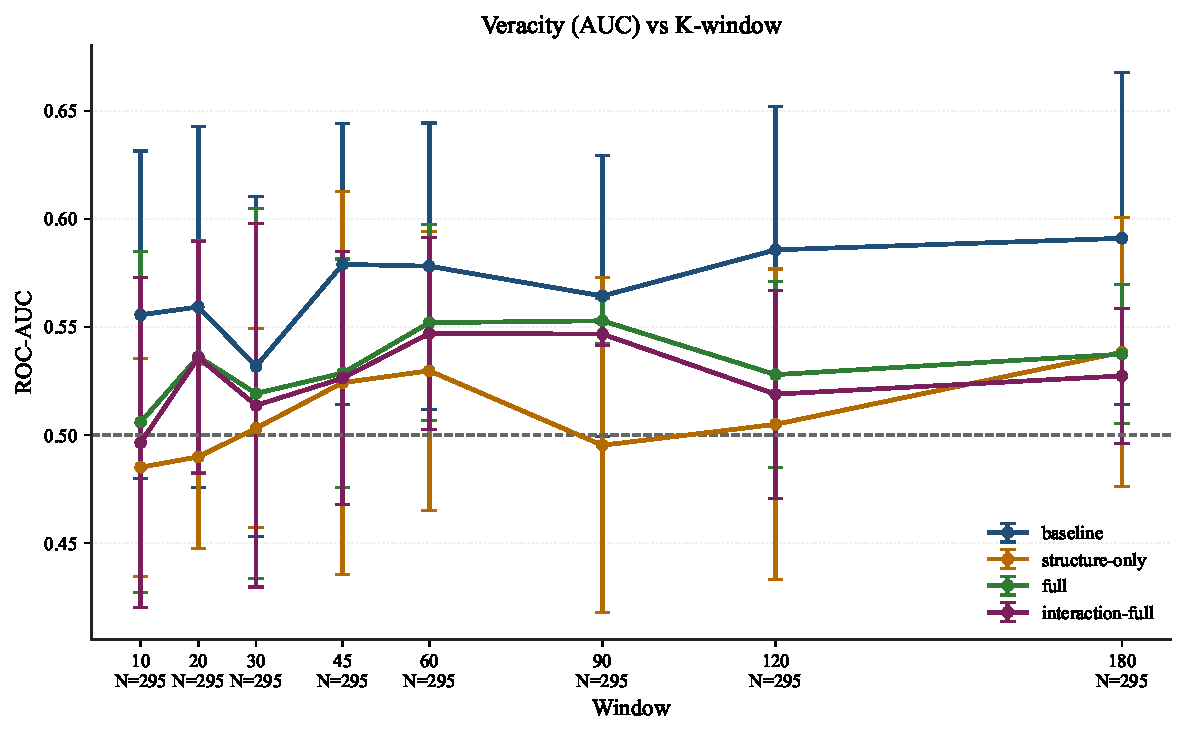
\includegraphics[width=0.8\linewidth]{Paper_sections/figures/F1K_k_veracity_primary.pdf}
  \caption{FibVID veracity (AUC) across size-based windows. Curves compare four bundles: baseline (tempo-only), structure-only (residualized structural shape features only; no tempo, dynamics, or interactions), full (baseline + structure + dynamics), and interaction-full (full + structure--tempo interactions). Error bars are 95\% CIs (from SE over fixed CV folds).}
  \label{fig:k_veracity_main}
\end{figure}

\begin{figure}[htbp]
  \centering
  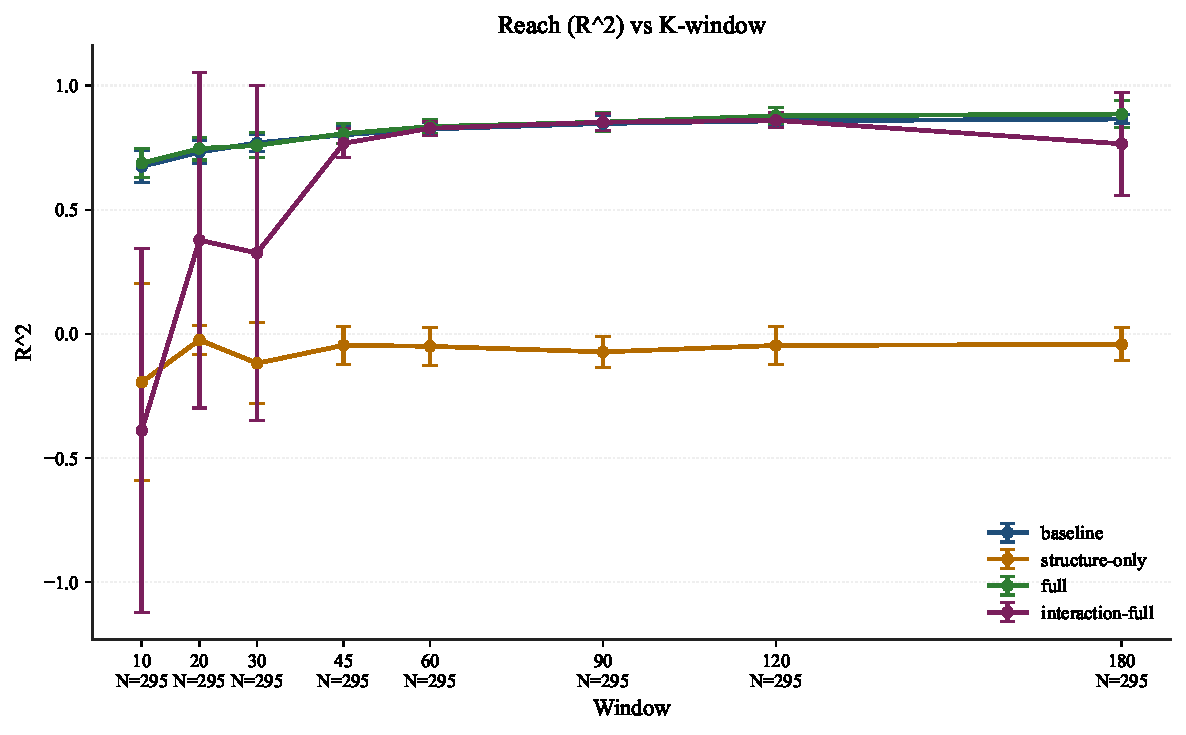
\includegraphics[width=0.8\linewidth]{Paper_sections/figures/F2K_k_reach_primary.pdf}
  \caption{FibVID reach prediction ($R^2$) across size-based windows with the same four bundles: baseline (tempo-only), structure-only (residualized structural shape features only; no tempo, dynamics, or interactions), full (baseline + structure + dynamics), and interaction-full (full + structure--tempo interactions). Error bars are 95\% CIs (from SE over fixed CV folds).}
  \label{fig:k_reach_main}
\end{figure}

The main pattern remains asymmetric across tasks, but it looks different from the earlier Twitter-only version. On FibVID, veracity performance is modest throughout. The strongest baseline logit result appears late rather than early, reaching AUC $\approx 0.591$ at $k=180$, while richer bundles do not improve consistently over that baseline. Reach is much stronger. Even simple baseline models perform well, and full bundles remain high throughout the larger windows, with OLS reaching $R^2 \approx 0.886$ at $k=180$ and the interaction-full specification peaking at about $R^2=0.861$ at $k=120$. In other words, early diffusion remains much more informative for eventual reach than for veracity. Table~\ref{tab:k_main_selected} reports selected baseline-vs-full comparisons at representative $k$ windows.

\begin{table}[htbp]
  \centering
  \caption{Selected FibVID $k$-window comparisons: baseline vs. full feature bundle (logit for veracity, OLS for reach).}
  \label{tab:k_main_selected}
  \begin{tabular}{rrrrrrr}
    \toprule
    $k$ & AUC (baseline) & AUC (full) & $\Delta$AUC & $R^2$ (baseline) & $R^2$ (full) & $\Delta R^2$ \\
    \midrule
    10  & 0.556 & 0.506 & -0.050 & 0.675 & 0.688 & +0.013 \\
    60  & 0.578 & 0.552 & -0.026 & 0.826 & 0.836 & +0.010 \\
    120 & 0.586 & 0.528 & -0.058 & 0.859 & 0.879 & +0.020 \\
    180 & 0.591 & 0.537 & -0.054 & 0.866 & 0.886 & +0.020 \\
    \bottomrule
  \end{tabular}
\end{table}

\subsection{Model Family Comparison and Incremental Gain}
Figure~\ref{fig:model_family_k} and Figure~\ref{fig:delta_gain_k} separate model-class effects from feature-bundle effects. Figure~\ref{fig:model_family_k} compares model families under the full bundle, while Figure~\ref{fig:delta_gain_k} shows incremental gain (full minus baseline) by model family. In Figure~\ref{fig:delta_gain_k}, bars above zero ($\Delta$AUC/$\Delta R^2 > 0$) mean full outperforms baseline; bars below zero indicate the opposite. On FibVID, the main takeaway is again task-specific. For veracity, model-class differences are limited and no model produces strong discrimination. For reach, all model families perform well at larger windows, with tree-based regressors especially strong in later windows. Table~\ref{tab:model_family_examples} summarizes model-family performance at representative early and late windows.

\begin{figure}[htbp]
  \centering
  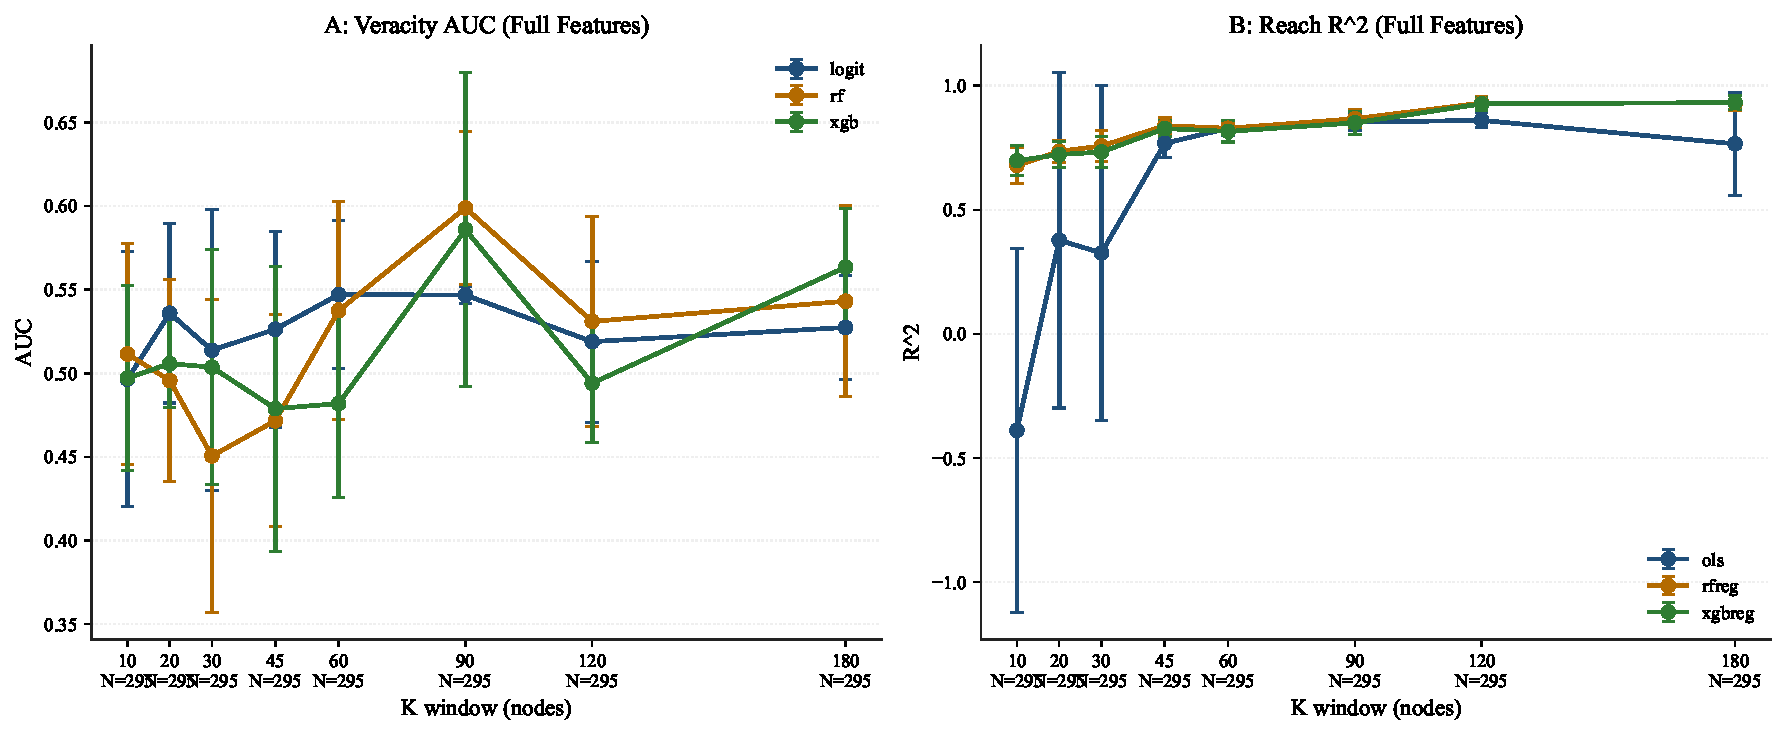
\includegraphics[width=0.95\linewidth]{Paper_sections/figures/F3_model_family_full_only.pdf}
  \caption{FibVID model-family comparison under the full feature bundle (residualized structure + dynamics + interactions) across $k$ windows.}
  \label{fig:model_family_k}
\end{figure}

\begin{figure}[htbp]
  \centering
  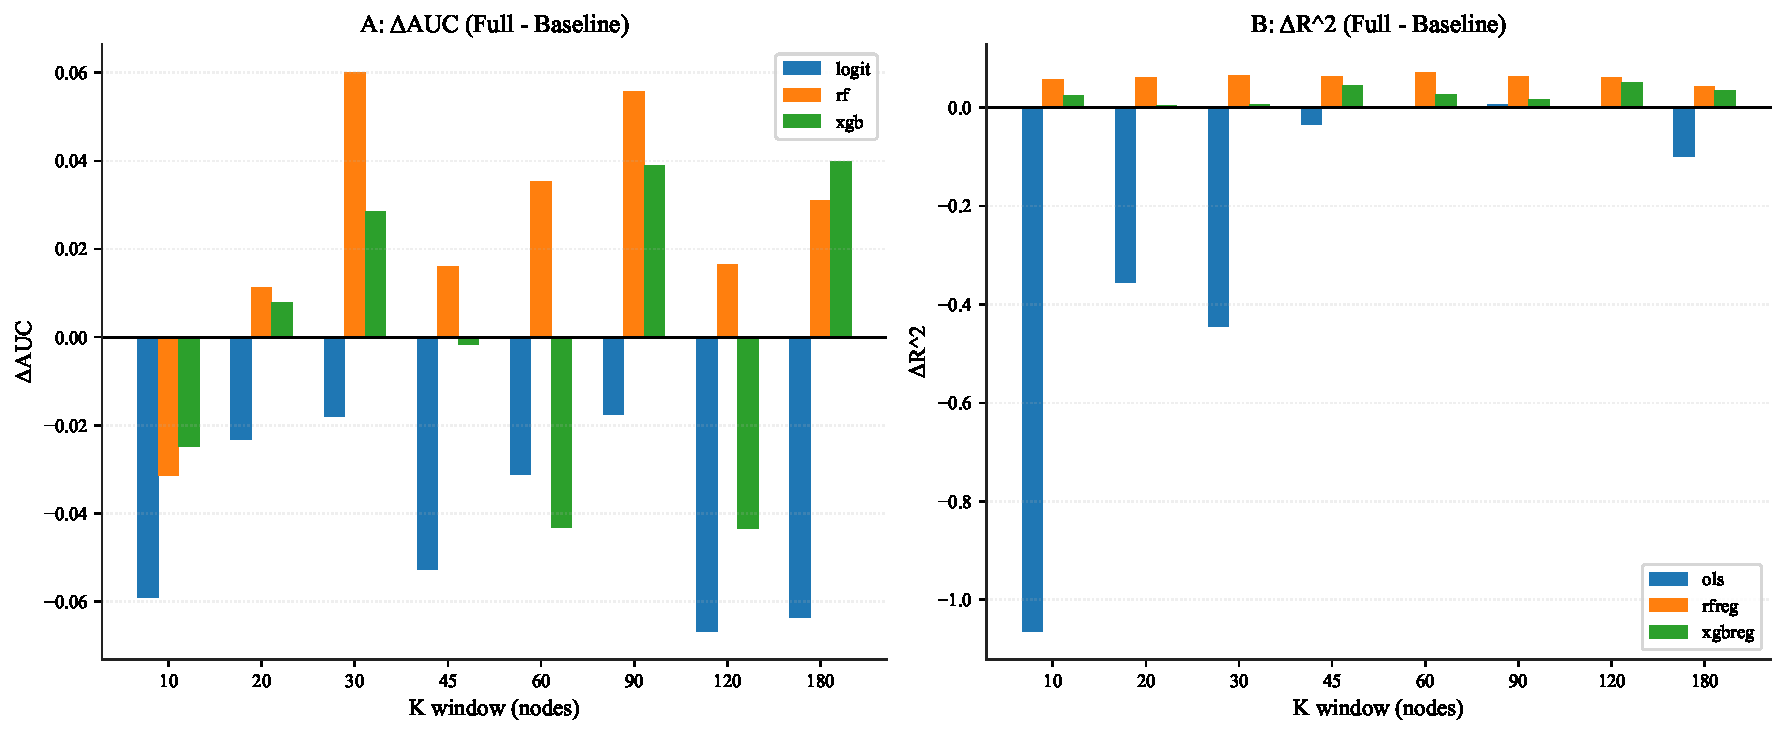
\includegraphics[width=0.95\linewidth]{Paper_sections/figures/F4_delta_gain_by_model.pdf}
  \caption{FibVID incremental gain (full minus baseline) by model family across $k$ windows; positive bars ($\Delta$AUC/$\Delta R^2 > 0$) indicate that full improves over baseline, while negative bars indicate degradation.}
  \label{fig:delta_gain_k}
\end{figure}

\begin{table}[htbp]
  \centering
  \caption{FibVID model-family comparison at representative early and late windows under the full feature bundle.}
  \label{tab:model_family_examples}
  \begin{tabular}{llrrrr}
    \toprule
    Window & Task & Logit/OLS & RF & XGB & Best \\
    \midrule
    $k=60$  & Veracity (AUC) & 0.547 & 0.537 & 0.482 & Logit \\
    $k=60$  & Reach ($R^2$)   & 0.829 & 0.829 & 0.816 & RF \\
    $k=180$ & Veracity (AUC) & 0.527 & 0.543 & 0.563 & XGB \\
    $k=180$ & Reach ($R^2$)   & 0.766 & 0.931 & 0.932 & XGB \\
    \bottomrule
  \end{tabular}
\end{table}

Two takeaways emerge. First, for veracity, linear logit remains competitive in mid windows, and the overall gains from greater model flexibility are limited. Second, for reach, tree-based regressors dominate late windows, indicating that non-linear effects matter much more for diffusion-outcome prediction than for veracity screening.

\subsection{Statistical Tests and Signal Validation}
Table~\ref{tab:k_paired_tests} reports paired fold-level $t$-tests comparing baseline vs. interaction-full models on FibVID. Figure~\ref{fig:perm_k60} provides permutation-based validation at $k=60$.

\begin{table}[!htbp]
  \centering
  \caption{Paired tests on FibVID (baseline vs. interaction-full): selected results from fixed 5-fold splits.}
  \label{tab:k_paired_tests}
  \begin{tabular}{rrrrr}
    \toprule
    Task & $k$ & Mean difference & $p$-value & Interpretation \\
    \midrule
    Veracity (AUC) & 10  & -0.0592 & 0.0518 & marginal negative \\
    Veracity (AUC) & 60  & -0.0311 & 0.2584 & null \\
    Reach ($R^2$)  & 60  & +0.0029 & 0.5735 & null \\
    Reach ($R^2$)  & 120 & +0.0021 & 0.8415 & null \\
    Reach ($R^2$)  & 180 & -0.1000 & 0.3815 & null \\
    \bottomrule
  \end{tabular}
\end{table}

\begin{figure}[!htbp]
  \centering
  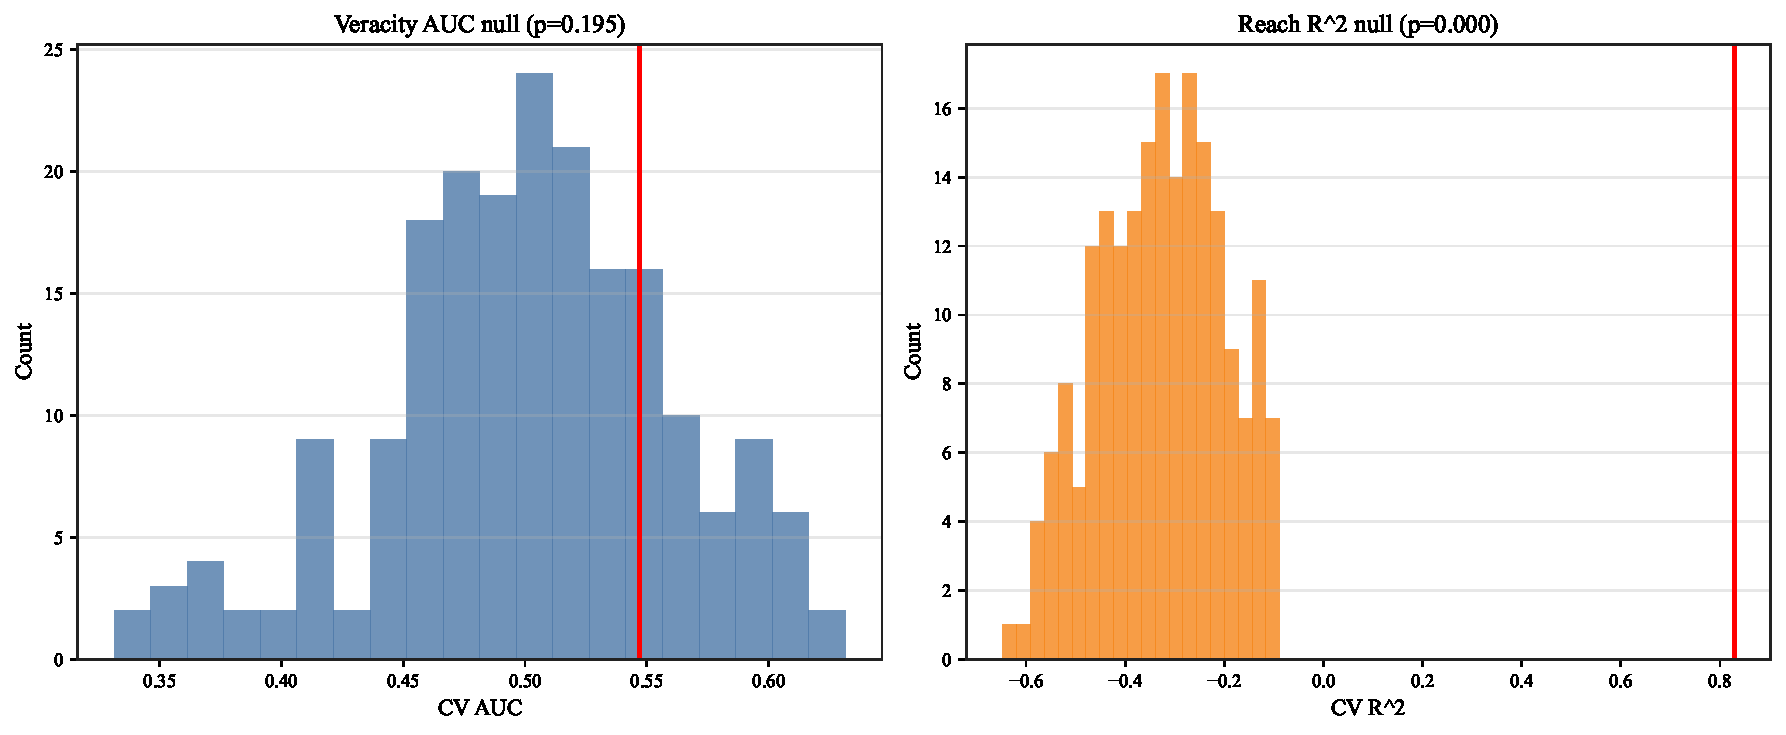
\includegraphics[width=0.88\linewidth]{Paper_sections/figures/F5_permutation_test_signal.pdf}
  \caption{FibVID permutation tests at $k=60$ (200 shuffles). Reach clearly exceeds the null, while veracity is only modestly separated from it.}
  \label{fig:perm_k60}
\end{figure}

The permutation results sharpen the task asymmetry. At $k=60$, observed reach $R^2$ is 0.829 versus a null mean of $-0.329$ (empirical $p=0/200$), which indicates a clear non-random signal. For veracity, observed AUC is 0.547 versus a null mean of 0.500, but the empirical $p$-value is 0.195. This is consistent with the earlier reading of the main figures: on FibVID, diffusion features are much more convincing for reach than for veracity.

\subsection{Comparative Benchmark: Twitter15/16}
The Twitter15/16 benchmark helps show which parts of the pattern carry over from the original rumor-tree setting. The basic asymmetry remains. Under the benchmark, the best interaction-full veracity result reaches AUC $\approx 0.657$ at $k=20$, while interaction-full reach reaches $R^2 \approx 0.719$ at $k=180$. Model-family comparisons in the benchmark also point in the same broad direction as FibVID: logit remains competitive for veracity in earlier windows, whereas tree-based regressors are stronger for reach, especially at larger $k$.

Relative to Twitter15/16, FibVID weakens the veracity side but strengthens the reach side. Put differently, the early-diffusion signal for reach appears stable and in this case even stronger on FibVID, whereas the signal for veracity remains modest in both datasets and is weaker on FibVID. The permutation tests show the same contrast. In Twitter15/16 at $k=60$, observed veracity AUC is about 0.640 against a null mean of 0.499, while observed reach $R^2$ is about 0.254 against a null mean of $-0.302$ (both empirical $p=0/200$). On FibVID, reach still clearly separates from the null, but veracity does not do so as strongly.

This comparison matters for interpretation. The Twitter benchmark shows that the original pipeline was capable of extracting some early veracity signal in a clean native tree setting. The FibVID results, however, make clear that this signal is limited and does not generalize as strongly as the reach result. That is why the final interpretation of veracity is more cautious: it is better read as a weak screening signal than as a strong classifier.

\begin{table}[htbp]
  \centering
  \caption{Summary of the main specifications reported in this section.}
  \label{tab:representation_summary}
  \begin{tabular}{p{3.5cm}p{3.3cm}p{2.3cm}p{2.3cm}}
    \toprule
    Specification & Role in results & Best veracity & Best reach \\
    \midrule
    FibVID harmonized $k$-window & Main analysis & AUC $\approx 0.591$ & $R^2 \approx 0.886$ \\
    Twitter15/16 $k$-window & Comparative benchmark & AUC $\approx 0.657$ & $R^2 \approx 0.719$ \\
    FibVID native graph & Supplementary veracity check & AUC $\approx 0.616$ & --- \\
    FibVID time-window & Robustness check & AUC $\approx 0.570$ & $R^2 \approx 0.396$ \\
    \bottomrule
  \end{tabular}
\end{table}

\subsection{Representation Sensitivity for Veracity}
\paragraph{Supplementary representation check for veracity.}
As a supplementary check, I also estimate veracity models on a native graph representation of FibVID that does not force claims into a single-root cascade. In that specification, the best veracity result reaches AUC $\approx 0.616$ at $W=180$. I treat this as a representation check rather than as a second main pipeline. It suggests that veracity may benefit from retaining more of the original claim-level topology, but it does not alter the main result of the paper, which is based on the harmonized cascade-compatible representation.

\subsection{Time-Window Robustness and Feature Diagnostics}
The time-window trajectory remains useful as a secondary diagnostic (Figure~\ref{fig:time_learning_curve}), especially for showing whether the main conclusions depend on the choice of window definition. On FibVID, the time-window results preserve the same qualitative ordering as the size-based analysis: veracity remains modest, while reach is still more predictable than veracity. The best time-window veracity result is around AUC $=0.570$ at $T=10$ under the interaction-full bundle, while the best full-bundle veracity result is around AUC $=0.545$ at $T=90$. For reach, the best full-bundle time-window result reaches about $R^2=0.396$ at $T=180$. This is far below the best size-based result on FibVID ($R^2 \approx 0.886$ at $k=180$), which supports keeping size-based windows as the main specification.

The same design logic also remains reasonable on the Twitter15/16 side. In the earlier benchmark analysis, time-window results were useful as a supplementary check on whether the main pattern depended on fixed-message windows alone, but they did not replace the size-based design as the primary specification. Taken together, the two datasets point in the same direction: time windows remain informative as a robustness check, but $k$-windows remain better suited to the main analysis because they hold observed information quantity fixed and recover much stronger reach signal.

\begin{figure}[!htbp]
  \centering
  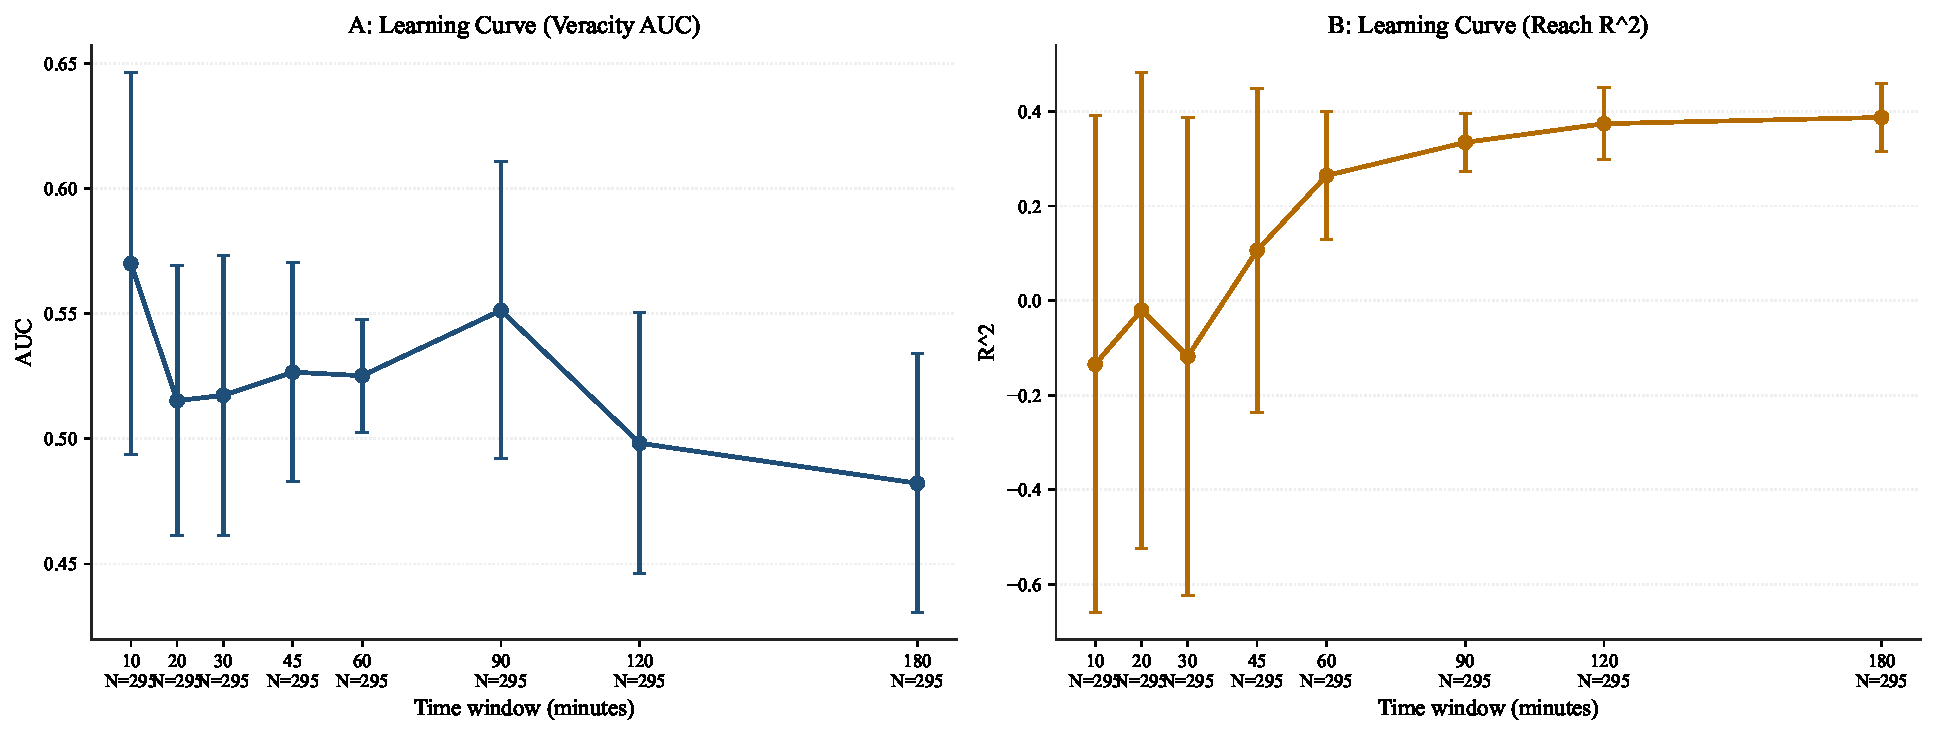
\includegraphics[width=0.92\linewidth]{Paper_sections/figures/F6_learning_curve_time.pdf}
  \caption{Supplementary FibVID time-window learning curves under the full dynamic+interaction feature bundle.}
  \label{fig:time_learning_curve}
\end{figure}

The residualization diagnostics in Table~\ref{tab:residualization_diag} show that first-order dependence of structural descriptors on log early volume is effectively removed. This remains important in the revised design because FibVID differs from Twitter15/16 not only in scale and class balance, but also in raw propagation format.

\begin{table}[!htbp]
  \centering
  \caption{Volume-dependence diagnostics before vs. after residualization (median absolute correlation with $\log(1+\text{early volume})$ over structural features).}
  \label{tab:residualization_diag}
  \begin{tabular}{lrr}
    \toprule
    Window type & Raw features & Residualized features \\
    \midrule
    Time windows & 0.248 & $\approx 3.5\times10^{-16}$ \\
    $k$ windows  & 0.103 & $\approx 1.0\times10^{-15}$ \\
    \bottomrule
  \end{tabular}
\end{table}
\FloatBarrier

\paragraph{Summary.}
Across tasks, the revised pipeline supports three conclusions: (1) size-based windows remain the strongest primary design; (2) early diffusion is much more informative for reach than for veracity on FibVID; and (3) Twitter15/16 remain useful as a benchmark, but the main substantive result is now anchored in FibVID rather than in the older rumor-tree dataset.
